\documentclass[ nooutcomes]{ximera}
\usepackage{fullpage}
\newcommand{\RR}{\mathbb R}
\renewcommand{\d}{\,d}
\newcommand{\dd}[2][]{\frac{d #1}{d #2}}
\renewcommand{\l}{\ell}
\newcommand{\ddx}{\frac{d}{dx}}
\newcommand{\dfn}{\textbf}
\newcommand{\eval}[1]{\bigg[ #1 \bigg]}

\usepackage{multicol}

\renewenvironment{freeResponse}{
\ifhandout\setbox0\vbox\bgroup\else
\begin{trivlist}\item[\hskip \labelsep\bfseries Solution:\hspace{2ex}]
\fi}
{\ifhandout\egroup\else
\end{trivlist}
\fi} 
\title{5.2: Definite Integrals}

\begin{document}
\begin{abstract}

\end{abstract}
\maketitle




%problem 1
\begin{problem}
Snow is starting to fall with a rate at any time $t$ after the start being 
$$ f'(t) = \frac{3}{2} t - \frac{1}{4} t^2 + \frac{3}{10} $$
inches per hour for $t$ in $[0,4]$ (i.e., the snow falls for 4 hours - from noon until 4pm).  
There were already $5$ inches of snow on the ground when the storm started.  
	\begin{enumerate}
	
	%part a 
	\item  Use the formula for a right Riemann sum to estimate how much snow fell during the storm using $n$ rectangles.
		\begin{freeResponse}
		$\Delta x = \frac{b-a}{n} = \frac{4-0}{n} = \frac{4}{n}$.
		
		$x_i = a + i \Delta x = 0 + i \frac{4}{n} = \frac{4i}{n}$.
			\begin{align*}
			f'(x_i) = f' \left( \frac{4i}{n} \right) &= \frac{3}{10} + \frac{3}{2} \left( \frac{4i}{n} \right) - \frac{1}{4} \left( \frac{4i}{n} \right)^2  \\
			&= \frac{3}{10} + \frac{6i}{n} - \frac{4i^2}{n^2}
			\end{align*}
			
		So our approximate area is:
			\begin{align*}
			\sum_{i=1}^n f'(x_i) \Delta x &= \sum_{i=1}^n \left[ \left( \frac{3}{10} + \frac{6i}{n} - \frac{4i^2}{n^2} \right) \left( \frac{4}{n} \right) \right]  \\
			&= \frac{4}{n} \sum_{i=1}^n \left( \frac{3}{10} + \frac{6i}{n} - \frac{4i^2}{n^2} \right)  \\
			&= \frac{4}{n} \sum_{i=1}^n \left( \frac{3}{10} \right) + \frac{4}{n} \sum_{i=1}^n \left( \frac{6i}{n} \right) - \frac{4}{n} \sum_{i=1}^n \left( \frac{4i^2}{n^2} \right)  \\
			&= \frac{6}{5n} \sum_{i=1}^n 1 + \frac{24}{n^2} \sum_{i=1}^n i - \frac{16}{n^3} \sum_{i=1}^n i^2  \\
			&= \frac{6}{5n} (n) + \frac{24}{n^2} \left( \frac{n(n+1)}{2} \right) - \frac{16}{n^3} \left( \frac{n(n+1)(2n+1)}{6} \right)  \\
			&= \frac{6}{5} + \frac{12(n+1)}{n} - \frac{8(n+1)(2n+1)}{3n^2}.
			\end{align*}
		\end{freeResponse}
		
		
		
	%part b
	\item  Take the limit as $n$ goes to infinity to find the exact amount of snow that fell.
		\begin{freeResponse}
			\begin{align*}
			&  \lim_{n \to \infty} \left( \frac{6}{5} + \frac{12(n+1)}{n} - \frac{8(n+1)(2n+1)}{3n^2} \right)  \\
			&= \lim_{n \to \infty} \left( \frac{6}{5} + 12 \left( 1 + \frac{1}{n} \right) - \frac{8(1 + \frac{1}{n})(2 + \frac{1}{n})}{3} \right)  \\
			&= \frac{6}{5} + 12(1 + 0) - \frac{8(1+0)(2+0)}{3}  \\
			&= \frac{6}{5} + 12 - \frac{16}{3} = \frac{18 + 180 - 80}{15} = \frac{118}{15}.
			\end{align*}
		\end{freeResponse}
		
		
		
	\end{enumerate}
	
\end{problem}

%problem 2
\begin{problem}
  Consider the following limit of (general) Riemann sums of a function $g$ on $[a, b]$:
  \[
    \lim_{\Delta \to 0} \sum_{k = 1}^n (x_k^* + \cos(x_k^*)) \Delta x_k\mbox{ , $[0, \pi]$.}
  \]
  Express the limit as a definite integral.
  \begin{freeResponse}
    We have 
    \[
      \int_0^\pi(x + \cos(x))\d x = \lim_{\Delta \to 0} \sum_{k = 1}^n (x_k^* + \cos(x_k^*)) \Delta x_k.
    \]
  \end{freeResponse}
\end{problem}

%problem 3
\begin{problem}
Let $f(x)$ and $g(x)$ be functions for which we only know the following:
$$ \int_1^4 f(x)\d x = 7	\qquad	\int_2^4 f(x)\d x = 5	\qquad	\int_1^4 g(x)\d x = 2 $$
Compute the following integrals, if possible.  If it is not possible, give examples explaining why not.
	\begin{enumerate}
	
	%part a 
	\item  $\int_1^4 (8f(x) - 7g(x))\d x $
		\begin{freeResponse}
			\begin{align*}
			\int_1^4 (8f(x) - 7g(x))\d x &= 8 \int_1^4 f(x) \d x - 7 \int_1^4 g(x) \d x  \\
			&= 8(7) - 7(2) \\
			&= 56 - 14 = 42
			\end{align*}
		\end{freeResponse}
		
		
		
	%part b
	\item  $\int_1^2 (-f(x)) \d x $
		\begin{freeResponse}
		First notice that
			\begin{equation*}
			\int_1^4 f(x) \d x - \int_2^4 f(x) \d x = \int_1^2 f(x) \d x.
			\end{equation*}
		So
			\begin{align*}
			\int_1^2 (-f(x)) \d x &= - \int_1^2 f(x) \d x  \\
			&= - \left( \int_1^4 f(x)\d x - \int_2^4 f(x)\d x \right)  \\
			&= - (7 - 5) = -2.
			\end{align*}
			
			%\begin{align*}
			%\int_1^2 (-f(x)) \d x &= - \int_1^2 f(x) \d x  \\
			%&= - \left( \int_1^4 f(x)\d x + \int_4^2 f(x)\d x \right)  \\
			%&= - \left( \int_1^4 f(x)\d x - \int_2^4 f(x)\d x \right)  \\
			%&= - (7 - 5) = -2
			%\end{align*}
		\end{freeResponse}
		
		
		
	%part c
	\item  $\int_1^4 \left| f(x) \right| \d x$
		\begin{freeResponse}
		We are not given enough information to solve this integral because we do not know the regions where $f$ is positive or negative.
		Consider the following two functions $f_1(x)$ and $f_2(x)$:  
		
		$f_1(x) =   \left\{ \begin{array}{cl}
	2		 	&	\qquad \text{if } \quad 1 \leq x < 2					\\
	\frac{5}{2}		&	\qquad \text{if } \quad 2 \leq x \leq 4		\end{array} \right.  $
	
	$f_2(x) =   \left\{ \begin{array}{cl}
	6		 	&	\qquad \text{if } \quad 1 \leq x < 1.5					\\
	-2		 	&	\qquad \text{if } \quad 1.5 \leq x < 2					\\
	\frac{5}{2}		&	\qquad \text{if } \quad 2 \leq x \leq 4		\end{array} \right.  $
	
	Just using geometry, one can check that
	$$ \int_1^4 f_1(x)\d x = 7	\qquad	\int_2^4 f_1(x)\d x = 5	\qquad	\int_1^4 f_2(x)\d x = 7	\qquad	\int_2^4 f_2(x)\d x = 5 $$
	and so both $f_1$ and $f_2$ satisfy the assumptions of $f$.  But notice that
	$$\int_1^4 \left| f_1(x) \right| \d x = 7	\qquad	\text{and}		\qquad	\int_1^4 \left| f_2(x) \right| \d x = 9  $$
	These two examples demonstrate that we were not given enough information to solve this problem.
		
		\end{freeResponse}
		
	%part d
	\item  $\int_1^4 \left( 2 - x + f(x) \right) \d x$
		\begin{freeResponse}
		First notice that since the integral is linear over addition:
			\begin{equation}\label{3d}
			\int_1^4 \left( 2 - x + f(x) \right) \d x = \int_1^4 2 \d x - \int_1^4 x \d x + \int_1^4 f(x) \d x = \int_1^4 2 \d x - \int_1^4 x \d x + 7.
			\end{equation}
		By using geometry, we can see that
			\begin{equation*}
			\int_1^4 2 \d x = 2(4-1) = 6
			\end{equation*}
			\begin{equation*}
			\int_1^4 x \d x = 1(4-1) + \frac{1}{2} (4-1)(4-1) = 3 + \frac{9}{2} = \frac{15}{2}.
			\end{equation*}
		Then substituting into equation \eqref{3d} gives:
			\begin{equation*}
			\int_1^4 \left( 2 - x + f(x) \right) \d x = 6 - \frac{15}{2} + 7 = \frac{11}{2}.
			\end{equation*}
		\end{freeResponse}
	\end{enumerate}
\end{problem}

%problem 4
\begin{problem}
  Evaluate the following sums:
  \begin{enumerate}
  \item $\sum_{i=1}^{4} i^5 $
    \begin{freeResponse}
      $\sum_{i=1}^{4} i^5 = 1^5 + 2^5 + 3^5 + 4^5 = 1 + 32 + 243 +
      1024 = 1300$.
    \end{freeResponse}

  \item $\sum_{i=1}^{400} (5(i+1)^2 + 3) $
    \begin{freeResponse}
      \begin{align*}
        \sum_{i=1}^{400} (5(i+1)^2 + 3) 
        &= \sum_{i=1}^{400} (5(i^2 + 2i + 1) + 3) \\
        &= \sum_{i=1}^{400} (5i^2 + 10i + 8) \\
        &= \sum_{i=1}^{400} 5i^2 + \sum_{i=1}^{400} 10i + \sum_{i=1}^{400} 8  \\
        &= 5\sum_{i=1}^{400} i^2 + 10 \sum_{i=1}^{400} i + 8(400)  \\
        &= 5 \left( \frac{400(400+1)(2(400) + 1)}{6} \right) + 10 \left( \frac{400(400+1)}{2} \right) + 3,200  \\
        &= 5 (200)(401)(267) + 10(200)(401) + 3,200  \\
        &= 107,067,000 + 802,000 + 3,200 = 107,872,200
      \end{align*}
    \end{freeResponse}
  \end{enumerate}
\end{problem}

%problem 5
\begin{problem}
  The \dfn{velocity} function for a man walking along a straight road which runs east and west is given by $v(t) = -t^2 + 4t - 3$ ft/min.
  \begin{enumerate}
    
  \item  Set up a definite integral for the man's \dfn{displacement} during the time interval from $2$ minutes to $6$ minutes after he began running.
    \begin{freeResponse}
      \begin{align*}
        \int_2^6 v(t) \d t &= \lim_{n \to \infty} \sum_{i=1}^n v(t_i) \Delta t
      \end{align*}
      Where:  \\	
      $\Delta t = \frac{b-a}{n} = \frac{6-2}{n} = \frac{4}{n}$.
      
      $t_i = a + i \Delta t = 2 + i \frac{4}{n} = 2 + \frac{4i}{n}$.
    \end{freeResponse}
    
  \item  \dfn{At home:}  Evaluate the definite integral using the limit of a right Riemann sum.
    \begin{freeResponse}
      \begin{align*}
        v(t_i) &= -\left(2 + \frac{4i}{n} \right)^2 + 4 \left( 2 + \frac{4i}{n} \right) - 3  \\
               &= - \left( 4 + \frac{16i}{n} + \frac{16i^2}{n^2} \right) + 8 + \frac{16i}{n} - 3  \\
               &= 1 - \frac{16i^2}{n^2}
      \end{align*}
      
      So we compute:
      \begin{align*}
        \int_2^6 v(t) \d t &= \lim_{n \to \infty} \sum_{i=1}^n \left[ \left( 1 - \frac{16i^2}{n^2} \right) \left( \frac{4}{n} \right) \right]  \\
                           &= \lim_{n \to \infty} \sum_{i=1}^n \left( \frac{4}{n} - \frac{64 i^2}{n^3} \right)  \\
                           &= \lim_{n \to \infty} \left[ \frac{4}{n} \sum_{i=1}^n 1 - \frac{64}{n^3} \sum_{i=1}^n i^2 \right]  \\
                           &= \lim_{n \to \infty} \left[ \frac{4}{n} (n) - \frac{64}{n^3} \left( \frac{n(n+1)(2n+1)}{6} \right) \right]  \\
                           &= 4 - \frac{64}{3} = \frac{12-64}{3} = - \frac{52}{3}.
      \end{align*}
    \end{freeResponse}
    
  \item  Is this the same as the total \dfn{distance} the man walked from $2$ minutes to $6$ minutes?
    Why or why not?
    \begin{freeResponse}
      This number is not the same as the total distance.
      The man starts his walk by going east (the positive direction) but eventually ends his walk west of where he started.
      
      The total distance that the man walks would be measured by computing 
      $$\int_2^6 \left| v(t) \right| \d t$$  
      \begin{image}
      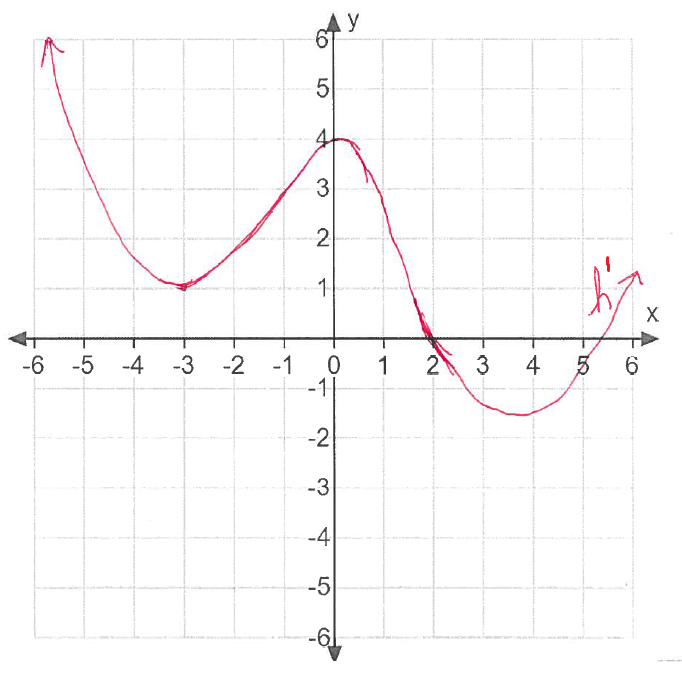
\includegraphics[scale=.7]{figure1.png}
            \end{image}
    \end{freeResponse}
  \end{enumerate}
\end{problem}


%problem 6
\begin{problem}
Use geometry to evaluate the definite integral.  Sketch the graph of the function and shade the relevant regions.
\begin{enumerate}


\item $\int_1^3 (2x-4) \d x$

\begin{freeResponse}
\begin{image}
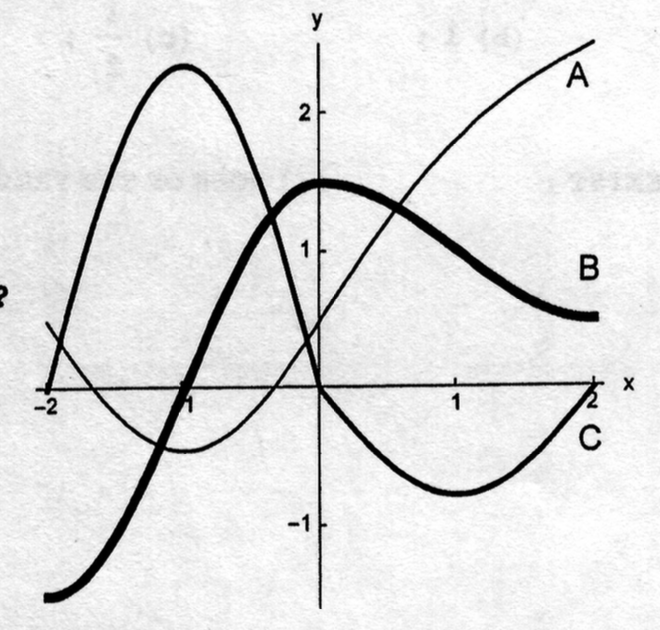
\includegraphics[scale=.4]{figure2.png}
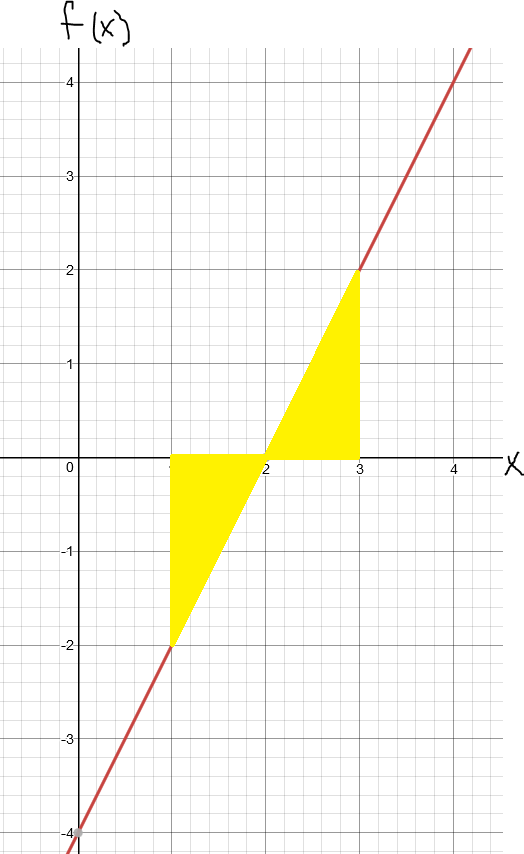
\includegraphics[scale=.4]{figure3.png}
\end{image}

We want to find the net area of the shaded region.  We have two identical triangles, each with base $1$ and height $2$.  Since the triangles will have identical area and one lies above and the other below the $x$-axis, the total area will be $0$.

Therefore, $\int_1^3 (2x-4) \d x=0$

\end{freeResponse}

\item  $\int_0^1 (2x-4) \d x$

\begin{freeResponse}
\begin{image}
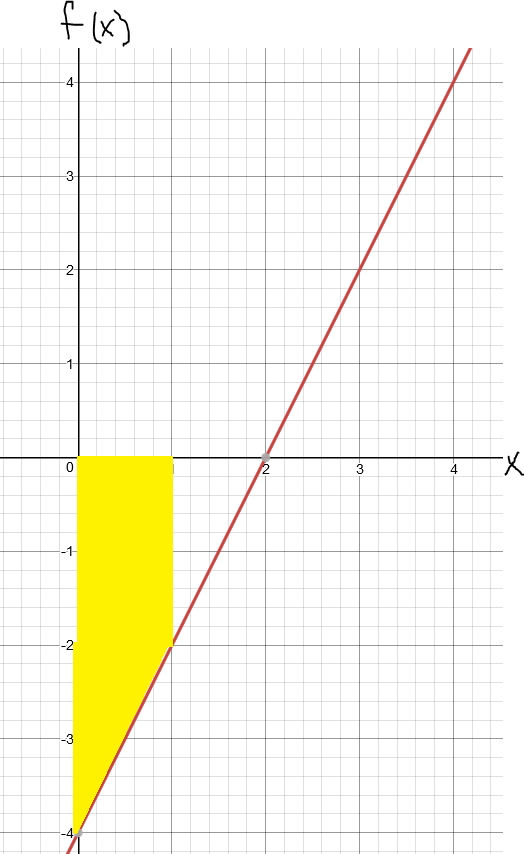
\includegraphics[scale=.35]{figure4.png}
\end{image}

Here we need to find the area of a trapezoid.  The trapezoid is made up of a rectangular top with area $(2)(1)=2$ and triangle bottom with area $(1/2)(1)(2)=1$.  This gives us an area of $3$, but, since $f$ is negative on the interval $(0,1)$, the value of the integral is the negative of this area.

Therefore,$\int_0^1 (2x-4) \d x=-3$


\end{freeResponse}
\item  $\int_{-1}^3 \sqrt{4-(x-1)^2} \d x$
\begin{freeResponse}

\begin{image}
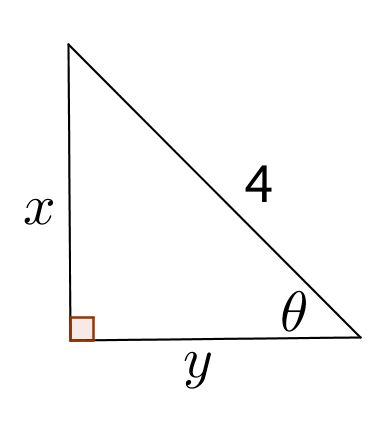
\includegraphics[scale=.4]{figure5.png}
\end{image}


We are looking for the area of the entire semi-circle above the $x$-axis.  This is a circle with radius $2$ so we have $(1/2)\pi 2^2=2 \pi$


$\int_{-1}^3 \sqrt{4-(x-1)^2} \d x= 2\pi$


\end{freeResponse}

\end{enumerate}
\end{problem}


\end{document} 
